\documentclass[CS4402-Notes.tex]{subfiles}
\begin{document}

\section{Search}
\subsection{Definitions}
\subsubsection{Systematic search}
The idea of \textbf{search} is to make an educated guess among several available alternatives, but be prepared to undo the guess and try a different alternative if the guess does not lead to a solution. 
\n
More concretely, \textbf{systematic} search is the case where given sufficient time:
\begin{itemize}
\item If there is a solution, it will be found
\item If there is no solution, the search space will be exhausted and the search will report that there is no solution
\end{itemize}
Typically, search is done through \textbf{partial assignments} of one or more decision variables which begins with an empty assignment and incrementally attempts to extend it into a solution. In this context, a \textbf{backtracking} search is one where if it is discovered that the current partial assignment cannot be extended to a solution (a dead end), then the algorithm backtracks over the last decision made and tries and alternative assignment. 

\subsubsection{Tree traversal}
The search for a solution to a CSP can be easily viewed as exploring a tree where the root represents the CSP with no assigned variables and each choice corresponds to the branches of the tree. 
\begin{figure}[H]
\centering
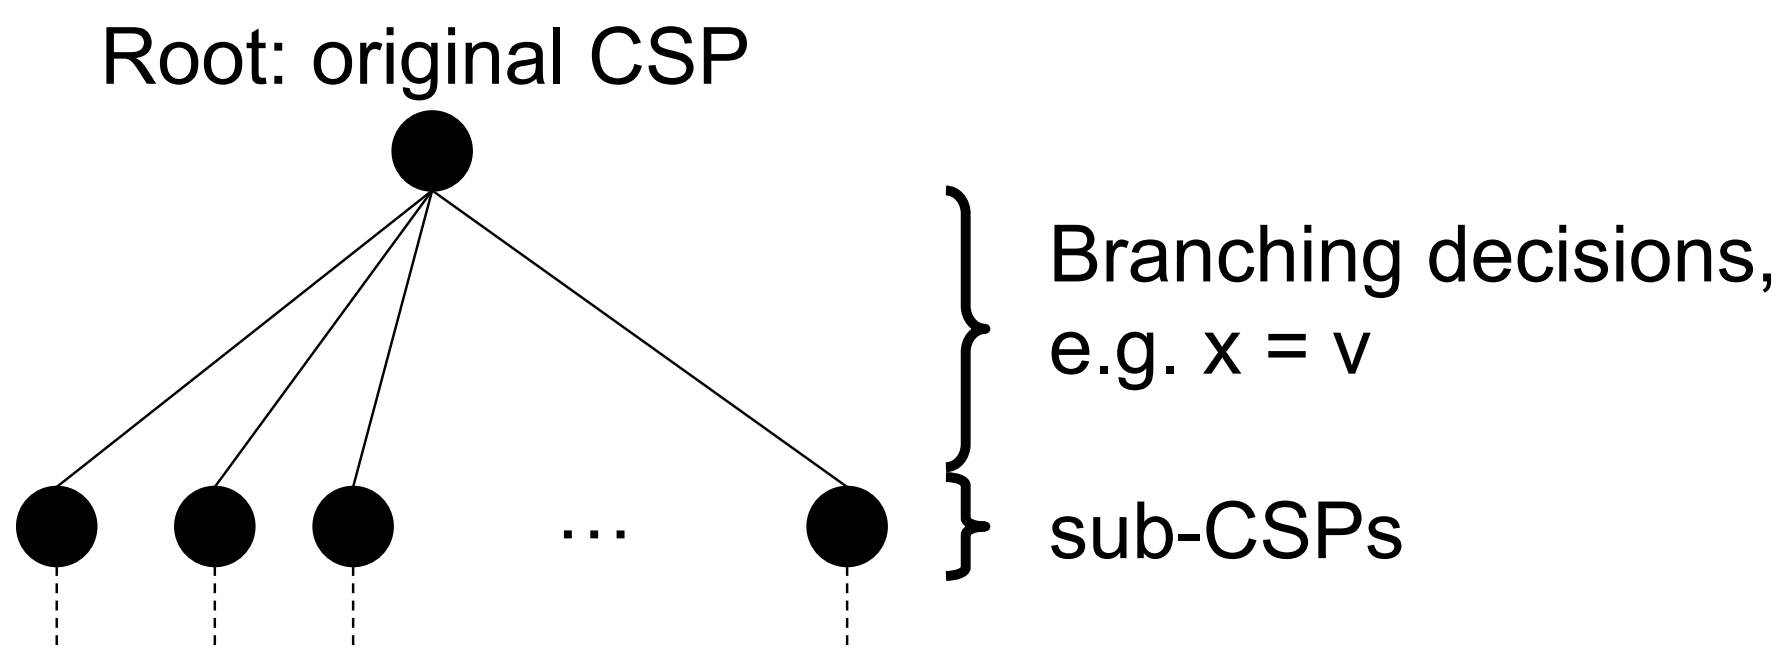
\includegraphics[width=0.85\textwidth, keepaspectratio]{imgs/csp-tree.png}
\caption{CSP search viewed as a tree.}
\end{figure}
\noindent
The descending nodes correspond to sub-CSPs which are the original CSP with partial assignments. Furthermore there are two common branching styles used for tree traversal: \textbf{d-way branching} and \textbf{2-way branching}.
\n
\textbf{D-way branching} \\
In d-way branching, each branch under the parent node represents the assignment of one of the $d$ domain values from the domain of a particular variable. For example, if $x \in \{1, 2, 3\}$, then there would be three branches which correspond to the assignment of $x$, one for each assignment. 
\n
\textbf{2-way branching} \\
\begin{figure}[H]
\centering
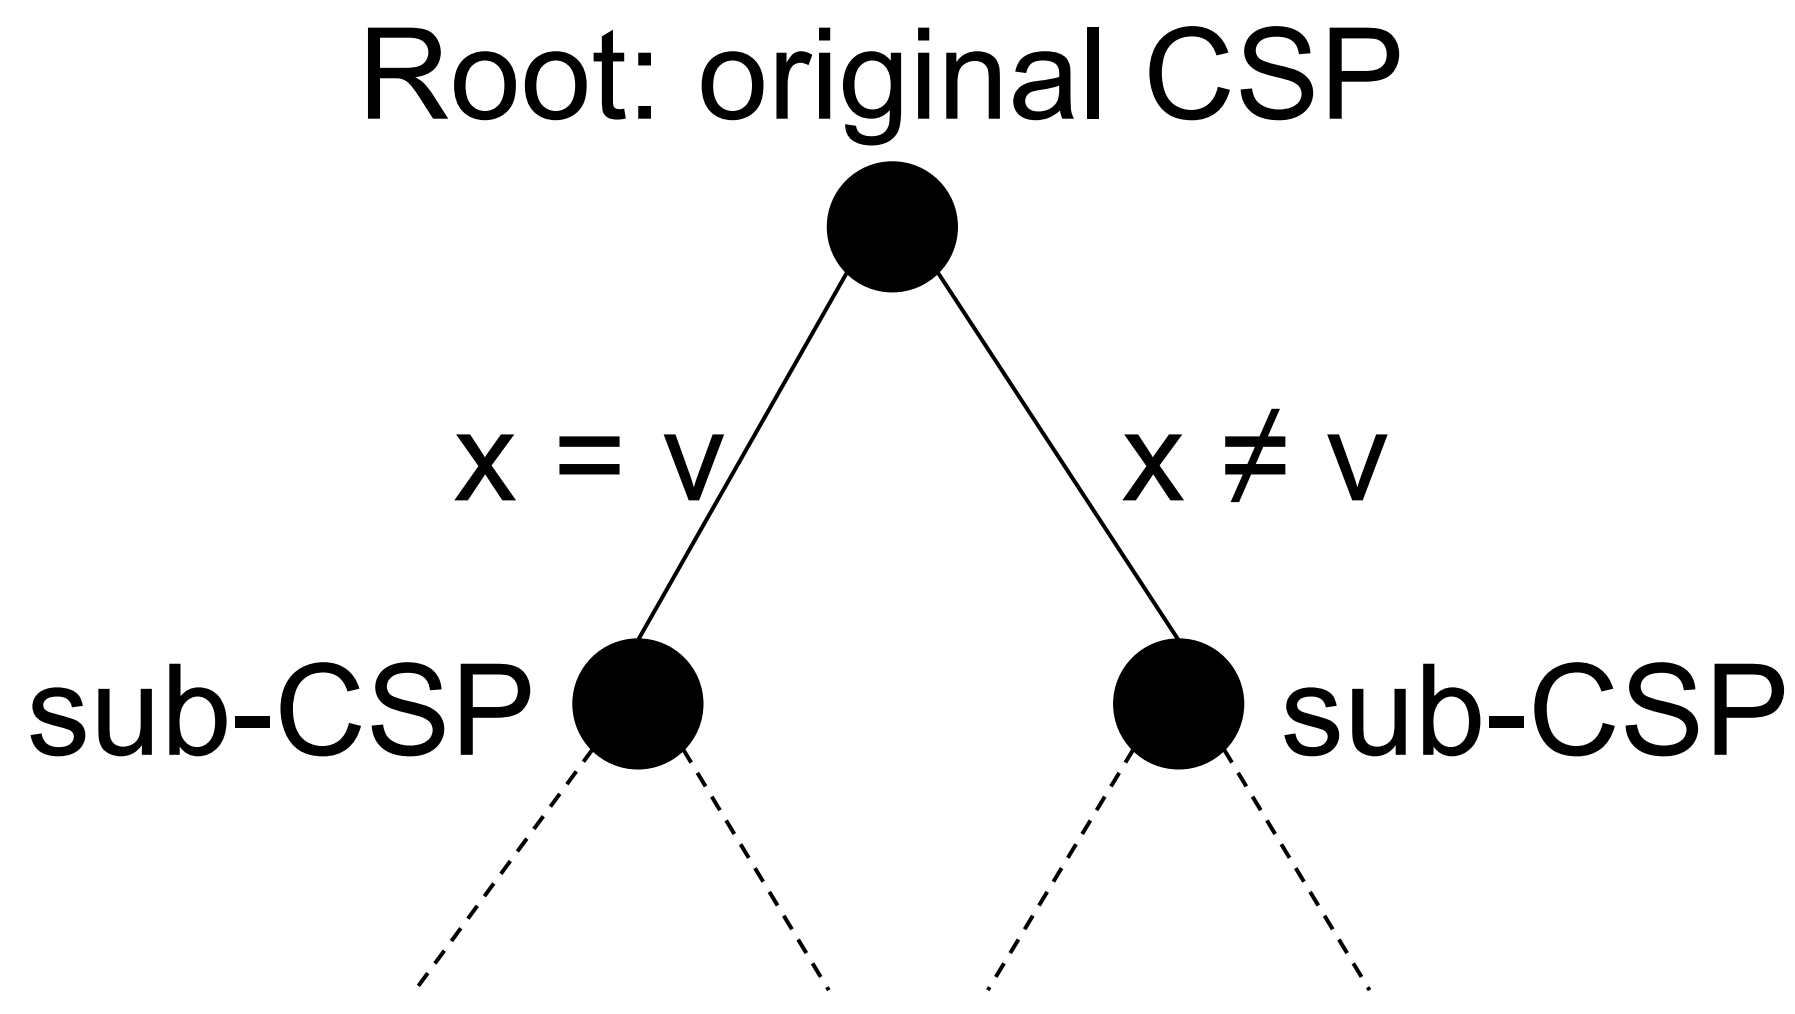
\includegraphics[width=0.4\textwidth, keepaspectratio]{imgs/2-way-branching.png}
\caption{2-way branching.}
\end{figure}
\noindent
In comparison, 2-way branching divides the search space into two pieces, one where the assignment to a particular domain value is true, and the other when it is false. The left branch tries to extend the partial assignment with $x = v$ first and if no solution is found down that branch, $v$ is removed from consideration entirely for the rest of the search. 

\subsubsection{Ordering}
In a search problem, there are both \textbf{variable orderings} and \textbf{value orderings}. They specify the order in which the variables are assigned and the order in which the values for the variables are tested. These can be either fixed or dynamic, depending on the heuristic. 
\n
Variables that have yet to be assigned are called \textbf{future} variables and similarly the variables that have been assigned are called \textbf{past} variables. 

\subsection{Methods}
\subsubsection{Generate and test}
Generate and test is a simple but very expensive method of solving a CSP. It is simply generating each \textbf{complete} assignment possible, then testing them all to see if any satisfy all the constraints. 
\n
This issue is further shown when trying to solve constraint \textit{optimisation} problems because simply satisfying the assignments is not enough it does not guarantee the best assignment. Therefore in this case, generate and test must examine all complete assignments except in the case where we know the current solution cannot be improved. 
\n
Simply put, generate and test is a brute force method that only checks constraints \textit{after} a complete assignment has been generated. It is systematic in that it is guaranteed to find a solution if one exists, however, due to its limitations in speed and memory it is never used in practice. 

\subsubsection{The backtrack algorithm}
The backtrack algorithm improves on generate and test by incrementally extending partial solutions. Every time an assignment is make, the constraints are checked to make sure none are violated.

\begin{algorithm}[H]
\begin{algorithmic}[1]
\Procedure{Backtrack}{\textit{depth}}
\For{\textit{d} in $D_{\text{depth}}$}
\State assign($x_{\text{depth}}$, \textit{d})
\State \textit{consistent} = TRUE
  \For{\textit{past} = 1 to \textit{depth} - 1 while \textit{consistent}}
    \State \textit{consistent} = text(constraint($x_{\text{past}}$, $x_{\text{depth}}$)
  \EndFor
  \If{\textit{consistent}}
    \If{\textit{depth} = \textit{n}}
      \State showSolution()
    \Else
      \State \textsc{Backtrack}(\textit{depth} + 1)
    \EndIf
  \EndIf
\EndFor
\EndProcedure
\end{algorithmic}
\caption{The backtrack algorithm}
\end{algorithm}
In the backtrack algorithm above, $D_{\text{depth}}$ is used to mean the domain fo the variable being assigned at the level \textit{depth}. After each assignment to a variable, all constraints with assigned variables are checked to ensure they are satisfied. If that all passes, then the algorithm either displays the solution or recurses. It is important to note that this algorithm will display \textit{all} solutions.
\n
In summary, the backtrack algorithm is a systematic search which guarantees to find a solution if one exists. It checks a constraint as soon as all of the variable that it constrains are instantiated. This allows it to spot dead-ends faster. In general, spotting dead-ends earlier leads to more search being saved.

\subsubsection{Branch and bound}
The branch and bound method is an augmented version of backtracking in order to find the best solution for optimisation problems. In this method, when a solution is reached, the value of the objective is recorded in $\alpha$. Then in any further search, if the partial assignment cannot improve over the current best value $\alpha$ then we backtrack immediately.
\n
In this case, there is a new function \texttt{calculateObjective()}, called the \textbf{bounding function} which calculates the lower bound on the objective from the current partial assignment. This assumes that any solutions extending the current partial assignment will have an objective calues equal to or greater than the current lower bound.
\begin{algorithm}[H]
\begin{algorithmic}[1]
\Procedure{BranchAndBound}{\textit{depth}}
\For{\textit{d} in $D_{\text{depth}}$}
\State assign($x_{\text{depth}}$, \textit{d})
\State \textit{objVal} = calculateObjective()
\If{objVal < $\alpha$}
\State \textit{consistent} = TRUE
  \For{\textit{past} = 1 to \textit{depth} - 1 while \textit{consistent}}
    \State \textit{consistent} = text(constraint($x_{\text{past}}$, $x_{\text{depth}}$)
  \EndFor
  \If{\textit{consistent}}
    \If{\textit{depth} = \textit{n}}
      \State $\alpha$ = \textit{objVal}
      \State showSolution()
    \Else
      \State \textsc{Backtrack}(\textit{depth} + 1)
    \EndIf
  \EndIf
\EndIf
\EndFor
\EndProcedure
\end{algorithmic}
\caption{The branch and bound algorithm}
\end{algorithm}
The branch and bound algorithm is also systematic, but further guarantees the \textit{best} solution, not just any solution. It checks constraints as soon as all of the variables that it constrains are instantiated, just like in backtrack and maintains the value of the objective associated with the current best solution so that we can backtrack sooner done every search path.

\subsection{Graphical representation}
It is often useful to view a CSP as a graph rather than a series of constraints and variables as it allows us to guide heuristics and propagation.

\subsubsection{Binary constraint graph}
In a binary constraint graph, each node represents a variable and the constraints are represented by the edges between the nodes. This only works for binary constraints because a constraint between more than three variables would not be able to be represented by an edge between nodes.
\begin{figure}[H]
  \centering
  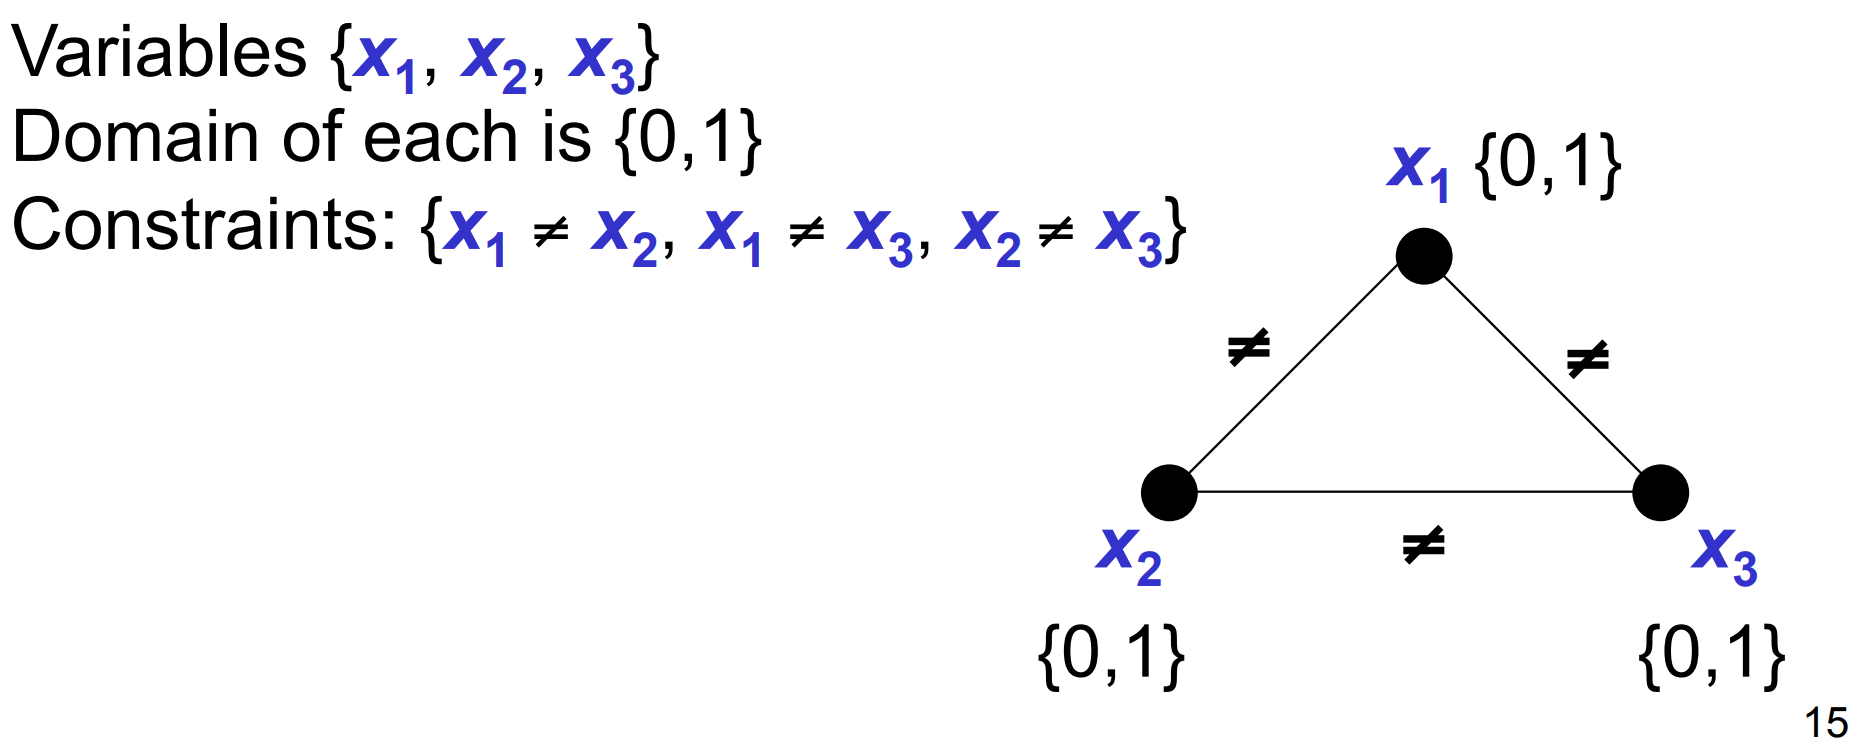
\includegraphics[width=0.8\textwidth, keepaspectratio]{imgs/binary-constraint-graph.png}
  \caption{Example of a binary CSP and its graphical representation.}
\end{figure}
\noindent
Because of the convenience of binary constraint graphs, we must find a way to turn non-binary instances into binary instances.

\subsubsection{Dual representation}
Dual representation is the method of transforming a non-binary CSP into a binary CSP. There are two simple steps to this conversion:
\begin{itemize}
\item Transform each constraint into a \textbf{dual variable} which has an associated domain of the allowed tuples
\item Add \textbf{binary constraints} between any two dual variables that share an original variable. These constraints insist that the assignments to the two nodes that it connects agree for the shared original variables.
\end{itemize}
For example, given the non-binary CSP with the following variables and constraints:
\begin{align}
  & x_1, x_2, x_3, x_4, x_5 \in \{0,1\} \\
  & x_1 + x_2 \neq x_3 \\
  & x_2 + x_3 \neq x_4 \\
  & x_3 + x_4 \neq x_5
\end{align}
We get the following tuples as the only valid assignments
\begin{equation}
y_1, y_2, y_3 \in \{\langle 0,0,1 \rangle, \langle 0,1,0 \rangle, \langle 1,0,0 \rangle, \langle 1,1,0 \rangle, \langle 1,1,1 \rangle \}
\end{equation}
However, tuples themselves cannot be used as domain elements as we think of domain values as \textbf{atomic}. Therefore, the tuples must be further transformed into an atomic value, the simplest method of which is to add up the values, which gives
\begin{equation}
y_1, y_2, y_3 \in \{1, 2, 4, 6, 7\}
\end{equation}
The graphical representation is just that same as in a typical binary constraint graph. Each node will represent a dual variable $y$ (an original constraint) and the edges between nodes corresponds to the new binary constraints which specify which of the original constraints share variables.

\section{Propagation}
Although backtracking in search is able to prune some parts of the search space, it is only looking backwards after an assignment has been made. However, we can be smarter than this to use constraints as a means of checking or pruning before actual assignments. This is known as \textbf{constraint propagation}, which deduces more information via a subset of the constraints. The deduced information can then be used to prune additional values from domains. 
\n
The idea is that local changes made form the basis for further deductions. Hence the result of a change is gradually \textit{propagated} through the constraint network.

\subsection{Consistency properties}
A consistency properties holds when constraint propagation of a certain kind reaches a \textbf{fixpoint}, in other words when nothing new can be deduced. Consistency may be either
\begin{itemize}
\item \textbf{Local} - one (or a subset of) constraints/arc/variables
\item \textbf{Global} - all constraints/arcs/variables
\end{itemize}

\subsubsection{Local node consistency}
Given a unary constraint $c(x_i)$, \textbf{local node consistency} holds if
\begin{equation}
\forall d \in D_i, c(x_1) \text{is satisfied when } x_i = d
\end{equation}
For example, given the constraint $x_1 < 5$ when $D_1 = \{3,4,5,6\}$, the node is not currently node consistent, so we can propagate $x_1 < 5$ to obtain $D_1 = \{3,4\}$ which is node consistent.

\subsubsection{Global node consistency}
Global node consistency is simply an extension of local node consistency which holds if local node consistency holds for \textit{all} unary constraints. It can be thought of as any single variable can be assigned a value from its domain consistently. Moreover, it can be enforced by simply enforcing node consistency for each unary constraint \textit{once}. 

\subsubsection{Local arc consistency}
As mention earlier, a constraint in a constraint graph is represented by an undirected edge between two nodes. For arc consistency, we consider splitting this up into \textbf{two directional arcs}
\begin{equation}
c(x_1,x_2) = arc(x_1,x_2) \wedge arc(x_2,x_1)
\end{equation}
Local arc consistency is then defined as follows:
\n
Given an arc $arc(x_i, x_j)$, local arc consistency holds if
\begin{itemize}
\item $c(x_i)$ and $c(x_j)$ are both node consistent
\item For each $d_i \in D_i$, there is at least one corresponding $d_j \in D_j$ such that $c(x_i, x_j)$ is satisfied when $x_i = d_i$ and $x_j = d_j$.
\end{itemize}
The propagation to maintain local arc consistency is known as \textbf{arc revision}. For example, given the arc $arc(x_1, x_2)$ of the constraint $x_1 < x_2$ and the two domains $x_1 \in \{2,11,16\}, x_2 \in \{2,5,10,11\}$, we can see that the values 11 and 16 in the domain of $x_1$ must be removed to maintain local arc consistency as they do not have any supporting values from the domain of $x_2$.
\n
\textbf{Supports} is the concept of \textit{evidence} that a domain value is consistent and therefore should not be removed. It is used in constraint propagation generally. In arc consistency, a support of a value in $x_1$ is a corresponding value in $x_2$ which satisfies the given constraint. For example, the values $\{5,10,11\}$ in the domain of $x_2$ support the value of $\{2\}$ in the domain of $x_1$ while $\{11,16\}$ had no supports and were removed.

\subsubsection{Global arc consistency}
Global arc consistency holds if local arc consistency holds for \textit{all} arcs. It can be thought of as any assignment to a single variable can be extended to an assignment to two variables consistently as global node consistency is a precondition.
\n
However, unlike global node consistency, it \textit{cannot} be enforced simply by enforcing local arc consistency for all arcs at once, as each time a domain has been pruned by one arc revision, connected arcs may no longer be consistent in the case that the only support is removed for some values.

\subsection{Enforcing arc consistency}
We know that it is not possible to enforce arc consistency in one pass in general, so algorithms are needed that an efficiently re-revise arcs as necessary. The goal is that after enforcing arc consistency, every arc in the problem is arc consistent. 

\subsubsection{AC1}
AC1 is the simplest method of enforcing arc consistency which is equivalent to a brute force method. The idea is to iterate passes of the revision of every arc until there are no more changes that need to be made. This is obviously inefficient as all arcs are revised regardless of the possibility of them having become inconsistent.

\subsubsection{AC3}
\begin{algorithm}[H]
\begin{algorithmic}[1]
\Procedure{AC3}{}
\For{$i = 1$ to $n$ \textsc{NC($x_1$)}}
\State $Q$ = allArcs($x_i, x_j$)
\While{not empty($Q$)}
    \State Remove any $arc(x_i, x_j)$ from $Q$
    \If{Revise($arc(x_i, x_j)$)}
        \State Add allArcs($x_h, x_i$) to $Q$ where $h \neq j$
    \EndIf
\EndWhile
\EndFor
\EndProcedure
\end{algorithmic}
\caption{The AC3 algorithm.}
\end{algorithm}
The algorithm of AC3 is explained following the pseudocode.
\n
3. The queue is first initialised with all arcs in the instance. \\
4. The termination condition is when there are no arcs left to revise, because all arcs are consistent at this point. \\
5. The order of processing is unimportant in order to find a final result, but the ordering can impact how much work is required. \\
6. Assuming that \textsc{Revise()} returns true if $D_i$ has been changed and also assuming empty domains are caught. \\
7. If $D_i$ changes, then we must re-revise arcs incident on $x_i$. Arcs that are already present to not have to be re-added as $Q$ is a set. The only exception is to not add the arc $arc(x_j,x_i)$.
\n
The reason $arc(x_j,x_i)$ does not have to be re-revised is because supports are \textbf{bi-directional}. That is to say if a value is supported on $arc(x_i,x_j)$, then it is supporting some value(s) on $arc(x_j,x_i)$. Conversely, if a value is not supported on $arc(x_i,x_j)$, then it is supporting no values on $arc(x_j,x_i)$ and therefore there is no need to revise $arc(x_j,x_i)$ after revising $arc(x_i,x_j)$.
\begin{algorithm}[H]
\begin{algorithmic}[1]
\Procedure{Revise}{$arc(x_i,x_j)$}
\State \textit{changed} = false
\For{$d_i$ in $D_i$}
\State \textit{supported} = false
\For{$d_j$ in $D_j$ while not supported}
\If{$x_i = d_i$, $x_j = d_j$ satisfies $c(x_i,x_j)$}
  \State \textit{supported} = true
\EndIf
\EndFor
\If{not \textit{supported}}
  \State Remove $d_i$ from $D_i$
  \State \textit{changed} = true
\EndIf
\EndFor
\If{empty($D_i$)}
  \State fail()
\EndIf
\State \Return \textit{changed}
\EndProcedure
\end{algorithmic}
\caption{Algorithm for the \textsc{Revise} function}
\end{algorithm}
Note that the worst case for AC3 is when the binary constraint graph is fully connected, as every arc other than the one currently being revised as to be added to the queue again whenever the domain changes.
\n
AC3 has a worst case time complexity of O($ed^3$) where $e$ is the number of edges in the constraint graph and $d$ is the maximum domain size. This is because each arc can only enter the queue at most $d$ times and there are $2e$ arcs, so \textsc{Revise} is executed O(ed) times. 

\subsubsection{AC4}
The issue with AC3 is that it is sub-optimal as it adds all arcs back to the queue whenever a variable's domain has been changed. This often wastes considerable effort in adding arcs onto the queue whose revision will not lead to any domain pruning and is the root cause of its sub-optimal time complexity of O($ed^3$). There are two approaches to reduce this issue and produce an optimal arc consistency algorithm.
\n
The idea is rather than having a corse-grained queue $Q$ of arcs to revise, we have a fine-grained list of deleted values $L$. This way, when revising an arc, it knows which value was deleted. AC4 is an example of such a fine-grained algorithm.
\n
In AC4, two additional structures are needed
\begin{itemize}
\item A \textbf{counter} is associated with \textit{each} arc-value pair $\langle arc(x_i,x_j), d_i \rangle$ where $d_i$ in $D_i$ which records the number of elements of $D_j$ that support $d_i$.
\item A \textbf{set} of pairs $\langle x_i, d_i \rangle$ associated with each $d_j$ in $D_j$ which records the assignments for which $d_j$ in $D_j$ provides support.
\end{itemize}
This way, for each domain element, we know how many supports it has, and for which other elements it provides support. This leads to the key aspect of AC4, which is to maintain a table of deleted domain values $M$ where $M[x_i, d_i]$ is 1 if deleted and 0 if otherwise and to maintain a list $L$ of deletions to propagate. The list $L$ contains individual value deletions rather than arcs.
\n
The algorithm has two phases, initialise and propagate.
\n
\textbf{Initialise} \\
\vspace{-0.5\baselineskip}
\begin{itemize}
\item Process each $arc(x_i, x_j)$ once
\item Enumerate support for each element in every domain $D_i$
\item If not support for $x_i = d_i$, then it is pruned and the list of deletions $L$ is initialised
\end{itemize}
\vspace{\baselineskip}
\textbf{Propagate} \\
\vspace{-0.5\baselineskip}
\begin{itemize}
\item Choose a deleted value to propagate from $L$
\item Iterate over the assignments supported by the deleted values ($S$)
\item Decrement their counters
\item If the counter reachers 0 and the element is not already deleted, delete and add to $L$
\item Repeat until arc consistency is established on all constraints (i.e., when $L$ is empty)
\end{itemize}
AC4 has a worst-case time complexity of O($ed^2$) where $e$ is the number of edges in the constraint graph and $d$ is the maximum domain size. O($ed^2$) time is needed for both the initialisation and propagation phase. In initialisation, for each arc is a double-nested loop of length d. In propagation, there are at most O($ed$) counters, each decremented at most $d$ times. This is worst-case optimal, it always reached the worst case because of the initialisation of the data structures. 
\n
Although AC4 has a better time complexity compared to AC3, it has a greater space complexity, requiring O($ed^2$) worst-case space complexity whereas AC3 only has a worst-case space complexity of O($e + nd$).

\subsubsection{AC2001/3.1}
The AC2001/3.1 algorithm adds the $Last$ data structure to the AC3 algorithm. This structure contains the last support in $D_j$ for $x_i = d_i$. This way, when revising the arc $arc(x_i, x_j)$ and checking the viability of $d_i$, the Last($arc(x_i, x_j), d_i$) can be checked to see if the last support is still present. If not, we only have to check for support in its successors.
\n
There is a subtle difference here in AC2001/3.1 compared to AC4. In AC4, for each value $d$, it is known which other values $d$ supports so that if $d$ is deleted, we need to ensure that there are other supports for that set. However in AC2001/3.1, only the last support found for $d_i$ is known. A key difference is AC2001/3.1 still uses \textsc{Revise} starting from the last support known.

\subsection{Forward checking}
Forward checking is a combination of propagation and search. It is the fundamental way in which systematic constraint solvers work and follows approximately the following steps:
\begin{enumerate}
\item Guess an assignment
\item Propagate consequences of that assignment
\item If all is well, back to step 1
\end{enumerate}
The basic idea is to revise arcs from every future variable to $x_i$ once after an assignment to $x_i$, which enforces local arc consistency on a subset of the arcs. This helps spot dead-ends earlier to reduce the amount of search.
\begin{algorithm}[H]
\begin{algorithmic}[1]
\Procedure{ForwardChecking}{\textit{depth}}
\For{$d$ in $D_{depth}$}
    \State assign($x_{depth}, d$)
    \State \textit{consistent} = true
    \For{\textit{future} = \textit{depth} + 1 to $n$ while \textit{consistent}}
        \State \textit{consistent} = \textsc{Revise($arc(x_{future}, x_{depth})$)}
    \EndFor
    \If{\textit{consistent}}
        \If{\textit{depth} = $n$}
            \State showSolution()
        \Else
            \State \textsc{ForwardChecking(\textit{depth} + 1)}
        \EndIf
    \EndIf
    \State undoPruning()
\EndFor
\EndProcedure
\end{algorithmic}
\end{algorithm}
Notice that forward checking does not require checking against the past variables, because the arc to the current variable was already checked when the past variable was assigned. This makes it so when considering an assignment to a current variable, all possible assignments are guaranteed to be compatible with the assignment to the past variable.
\n
Forward checking is complete and guarantted to find a solution if one exists. It is also guaranteed to explore a search tree that is \textit{smaller than or equal-sized} to that of backtrack. This saves search compared to backtrack whenever there is a domain wipeout of a future variable. Finally, forward checking can be combined with branch and bound for optimisation problems to result in better information about the objective and better propagation of the current best value. 

\subsubsection{Non-binary forward checking}
We wish to also extend forward checking to non-binary constraints and continue to achieve arc consistency on a set of constraints involving past and future variables. The algorithm for this is \textbf{nfc0}.
\begin{itemize}
\item After an assignment to $x_i$, make the constraints involving $x_i$, one future variables and any number of past variables consistent in one pass
\item This is like in binary forward checking, except that we must wait until \textit{all but one} variable in a constraint has been assigned before any propagation
\end{itemize}


\subsection{Look-back schemes}
In look-ahead schemes like forward checking and maintaining arc consistency are invoked when an algorithm is preparing to extend the current partial assignment. This also includes the variable/value ordering heuristics. In contrast, \textbf{look-back} schemes are invoked when a dead-end is encountered and the algorithm must backtrack.
\n
There are two types of lock-back schemes:
\begin{itemize}
\item Conflict recording - functions that add new constraints to prevent the same conflicts re-occurring
  \item Backjumping - functions that decide how far to backtrack by analysing the reasons for the dead-end
\end{itemize}

\subsubsection{Backjumping}
The idea of backjumping is to replace the simple backtracking algorithm with a \textbf{jump} back to the variable that is causing the dead-end. How this variable is determined depends on the look-forward scheme (eg, backtrack or forward checking). We shall focus on the case using backtracking as the look-foward scheme.
\n
Assuming that we have checked the past variables in order of assignment, backjumping records the \textbf{maxCheckLevel}, the deepest level that a check is made against when assigning $x_{\text{depth}} = d$. Then the \texttt{returnDepth} is the deepest \texttt{maxCheckLevel} for all $d$ in $D_{\text{depth}}$ where deepest means the largest number. These two variables are local to the search node where $x_{\text{depth}}$ is assigned.
\n
When the domain of $x_{\text{depth}}$ is exhausted, we jump back to \texttt{returnDepth}. The intuition behind this is if we exhausted $D_{\text{depth}}$ without checking assignments to variables deeper than \texttt{returnDepth}, these variables are clearly not part of the conflict.
\n
The issue with basic backjumping is that after a single jump, it resorts to chronological backtracking. This is because it jumps back to the maximum level checked against. If an assignment to $x_{\text{depth}}$ is consistent, checks must have been made up to $x_{\text{depth}-1}$. Because of this limitation, backjumping is often not very useful. Moreover, using the dynamic smallest domain variable order, backjump will visit exactly the same nodes as backtracking.

\subsubsection{Max-fail backjump}
Instead of jumping back to only the last checked level, we could try to jump back to the maximum level that \textbf{failed a check}. However, this does not work as it leads to incompleteness. Jumping back that far could lead to jumping back over a potential solution.

\subsubsection{Conflict-direction backjumping}
What can be done instead is to maintain a set of assignments failed against when trying new assignments. Then, then jumping back from $x_j$, to $x_i$, we can \textbf{combine} their conflict sets, which avoids forgetting other assignments that were conflicting with $x_j$ and also allows for multiple backjumps.
\n
The conflict set contains the set of past variables with which a conflict was found when attempting to assign $x_i$. Each \texttt{conflictSet$_i$} is local to a search node. The \texttt{returnDepth} is now the deepest variable in the conflict set.

\subsection{Heuristics}
Heuristics for CSP/COPs are rules of thumb that can be followed, which usually is expected to lead to an improvement. There are two different operations which we can order heuristically when trying to solve a constraint problem:
\begin{itemize}
\item Variable assignment order
\item Value assignment order
\end{itemize}
In particular, the perfect heuristic for value assignment will lead \textit{directly} to a solution.
\n
There are also two different forms heuristics can come in, \textbf{static} and \textbf{dynamic}. Static heuristics are ones in which the order is chosen before the search begins and is fixed for the entire search. Dynamic heuristics work the other way around where the state of the problem is examined and the best variable/value to assign next is decided based on the current state.
\n
The variable ordering during search can have a significant effect on the speed of the search. In particular, inefficient variable ordering leads to lots of thrashing, where repeated failures occur for the same reason because of the variable order. The rationale is therefore to make the \textbf{most difficult} choice first, which is likely to have the most far-reaching consequences for the rest of the problem. This has the added effect of narrowing down easy choices. 

\subsubsection{Static variable order heuristics}
There are three static variables heuristics we will look at, all three require a graph to represent the constraints called the \textbf{primal graph}. The primal graph has an edge between two variables iff they are in a constraint together. Unlike the constraint graph, where each edge represents one constraint.
\begin{figure}[H]
  \centering
  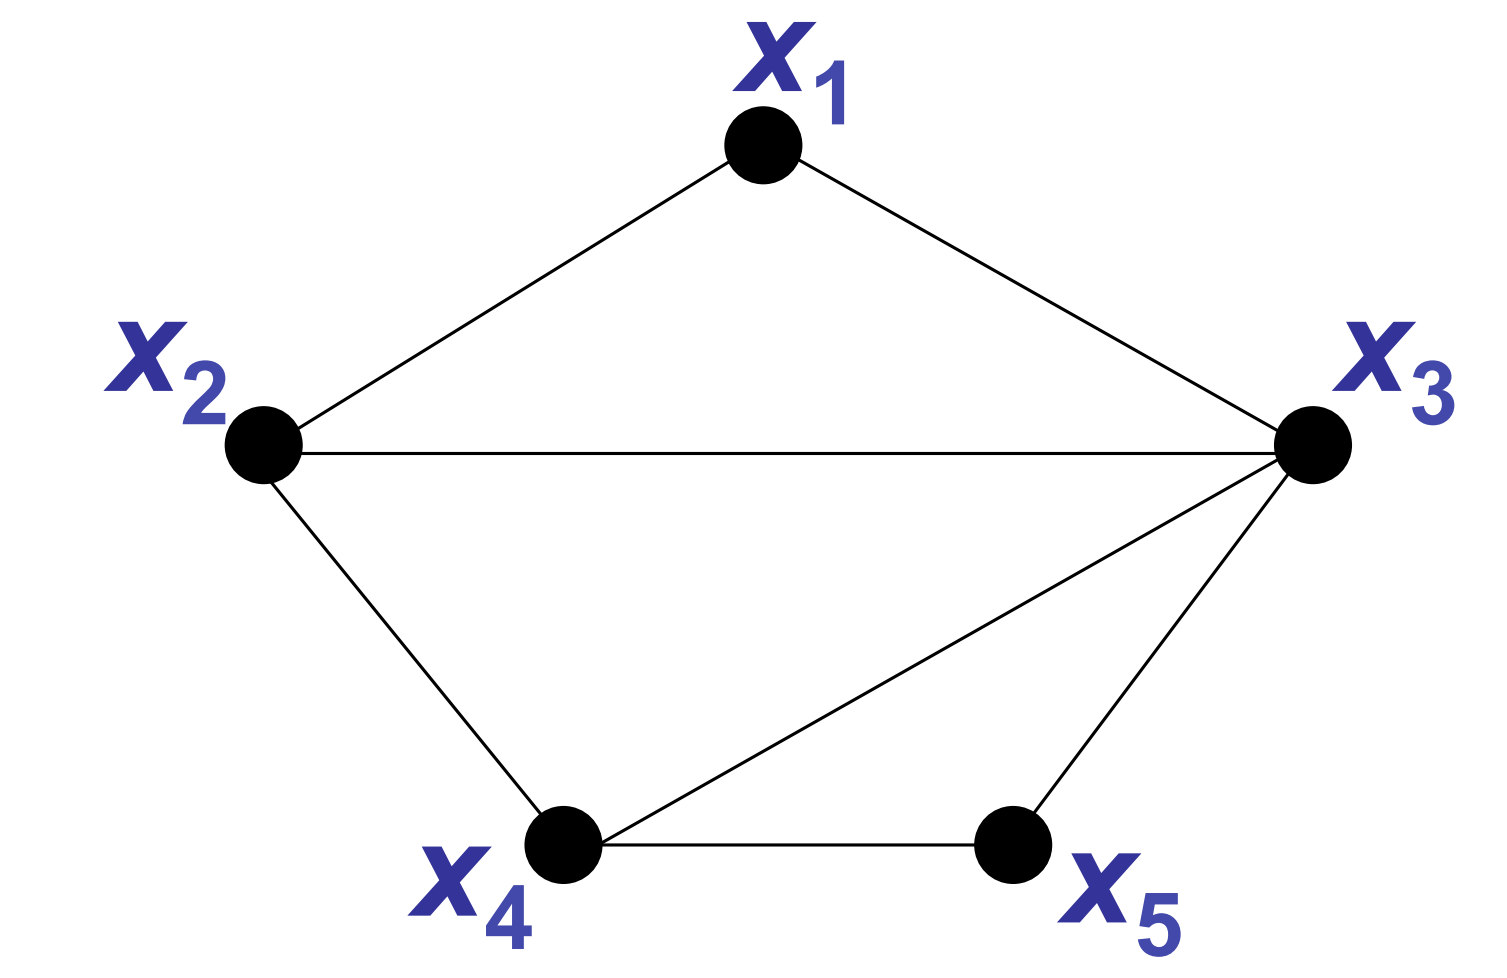
\includegraphics[width=0.5\textwidth, keepaspectratio]{imgs/primal-graph.png}
  \caption{Example of a primal graph for the CSP with the three constraints $c(x_1,x_2,x_3), c(x_2,x_3,x_4), c(x_3,x_4,x_5)$}
\end{figure}
\noindent
\textbf{Maximum degree}\\
The maximum degree heuristic orders the variables in decreasing order of their degrees in the graph. Any ties with the same order are chosen arbitrarily. This follows the rationale of choosing the most difficult choice first as variables that are part of a lot of constraints are more highly constrained and highly constrained variables may be the hardest choices. 
\n
\textbf{Maximum cardinality} \\
In maximum cardinality, the first variable is selected arbitrarily and the next variable is the variable connected to the largest group among those already selected. The idea behind this is after assigning some variables, we reason that the next hard choice is the one most constrained by the existing assignment as we need to make choices compatible with the existing assignment.
\n
\textbf{Minimum width} \\
The minimum width heuristic uses an ordered graph, which is an arrangement of graph nodes into a fixed linear order. The \textbf{width} at an ordered node is defined as the number of arcs linking back to a previous node in the order. The width of an ordering is the maximum width at any node and the width of a graph is the minimum width of all its orderings. To use this heuristic, the minimum width of the graph and an ordering corresponding to this width.

\subsubsection{Dynamic variable order heuristics}
\textbf{Smallest domain first} \\
Smallest domain first selects the variable with the smallest number of values compatible with past assignments. This is dynamic rather than static because the selection is made based on the state \textit{during} the search. As such, different branches of the search tree can have different variable orders. 
\n
\textbf{Brelaz} \\
The Brelaz heuristic selects the variable with the smallest number of values compatible with past assignments just like smallest domain first. The difference is that to break ties, the variable with the maximum degree in the constraint sub-graph of the future variables is chosen. 
\n
\textbf{dom/deg} \\
domdeg

\subsubsection{Value assignment order}
\textbf{Min-conflicts}
asd
\n
\textbf{Geelen's value-ordering heuristics}
\subsubsection{Variable order}

\subsubsection{Value order}

\subsection{Maintaining arc consistency}
While forward checking performs just sufficient propagation that it no longer needs to check backwards, we could do better by imbedding arc consistency algorithms into a search to enforce arc consistency. This leads us to the idea of \textbf{MAC} (Maintaining Arc Consistency).
\n
The basic idea is to always make sure the partial assignments made continue to have global arc consistency. After every assignment, global arc consistency must be re-established. This gives the benefits of spotting dead-ends earlier than forward checking and is relatively efficient as long as an efficient arc consistency algorithm is used.
\n
To do this, it is not necessary to revise all arcs at every node on a branch of the search tree. The trick is to think of assigning a value to a variable as saying that variable only has the domain with that one value and running a standard arc consistency algorithm on it. MAC also uses two way branching as it allows arc consistency to be established on the right branch after the value removal. After every left branch $x_i = d_i$, the queue is initialised with the consequences of removing all but $d_i$ from $D_i$, which propagates these changes to re-establish arc consistency. The right branch is handled similarly. 


\subsection{Conflict recording}
Conflict recording is like a form of learning constraints as we solve the CSP. The idea is that when a dead-end is encountered, a new constraint is created to stop that dead-end from re-occurring. This information is recorded for later use. There is no point adding a constraint for the exact constraint of dead-end assignments as it will never occurr again (known as a \textbf{nogood}). However, the conflict set could contain subsets that are conflict sets with other variables that have not been assigned yet. If we can identify these subsets, the appropriate nogoods can be added to prevent conflicts from re-occurring.

\subsubsection{Graph based learning}
We can visualise the order of assignments as a graph, so that when reaching dead-end on one node, we can blame the parent assignment to formulate the nogood. Because graph based learning blames adjacent variables that are assigned by search for a domain wipeout, it cannot be used with MAC.

\subsubsection{Value based learning}
Value based learning is a refinement of graph based learning. Rather than blaming only the parent node, we say past variables whose assignments are compatible with \textbf{all} elements of $D_i$ are irrelevant.

\subsubsection{Jump-back learning}

\subsection{Path consistency}
Rather than just checking the consistency between two nodes in arc consistency, the consistency between three nodes can be checked in \textbf{path consistency}

\subsubsection{Local path consistency}
Local path consistency is defined as a constraint $c(x_i, x_j)$ is path consistent with respect to a third variable $x_k$ iff for every pair $\langle d_i, d_j \rangle$ satisfying the constraint, there exists $d_k \in D_k$ such that $\langle d_i, d_k \rangle$ satisfies $c(x_i, x_k)$ and $\langle d_j, d_k \rangle$ satisfies $c(x_j, x_k)$.
\n
To enforce local path consistency, the revision step is as follows:
\begin{itemize}
\item Given $c(x_i, x_j)$ and $x_k$
\item For each tuple $\langle d_i, d_j \rangle$ satisfying $c(x_i, x_j)$
  \begin{itemize}
  \item If no value $d_k \in D_k$ exists such that $\langle d_i, d_k \rangle$ satisfies $c(x_i, x_k)$ and $\langle d_j, d_k \rangle$ satisfies $c(x_j, x_k)$
  \item Then remove $\langle d_i, d_j \rangle$ from the set of satisfying tuples $c(x_i, x_j)$.
  \end{itemize}
\end{itemize}
It is important to notice that previous when enforcing arc consistency, we were removing values from domains, which is equivalent to adding unary constraints to the node $x_i \neq v$. Here, we are adding a binary constraints $c(x_i, x_j)$ due to having no valid assignment in $x_k$ that support that tuple $\langle d_i, d_j \rangle$.
\n
There are algorithms for enforcing path consistency similar in structure to hose for enforcing arc consistency. Finally, path consistency implies arc consistency just as arc consistency implies node consistency. We can see a pattern developing here:
\begin{itemize}
\item Node consistency - Can assign a value to any one variable consistently
\item Arc consistency - Given a constraint assignment to any one variable, can extend it to two variables consistently
\item Path consistency - Given a consistent assignment to any two variables, can extend it to three variables consistently
\end{itemize}

\subsection{K-consistency}
K-consistency is the generalised application of consistency for up to $k$ nodes. It holds iff:
\begin{itemize}
\item Given assignments to $k - 1$ variables, satisfying all constraints among them
\item Can choose an assignment to any $k$th variable such that constraints among all $k$ variables are satisfied
\end{itemize}
Strong k-consistency is defined as $j$-consistency for all $1 \leq j \leq k$. In more detail
\begin{itemize}
\item Given any set $X$ of $k - 1$ variables with constraints $C_X$ whose scopes are contained within $X$ (i.e. no constraints with some variables in $X$, others not)
\item For all assignments $A$ to $X$ that satisfy the constraints in $C_X$ and the variable domains:
\item For all variables $x_k$ not in $X$:
\item $A$ can be extended to $x_k$ without violating any constraint with scope contained in $X + \{x_k\}$.
\end{itemize}
Further, $k$-consistency does not require binary CSPs. 


\end{document}
